\newpage
\section{Metodologia Experimental}

    \subsection{Atividade 1 – Circuitos Ressonantes}
        O primeiro experimento consistiu na análise do circuito ressonante 
        paralelo mostrado na figura 4. Primeiramente calculamos a frequência de 
        ressonância do circuito a partir da equação 1 mostrada anteriormente. 
        Com a simulação realizada utilizando o software OrCAD, encontrou-se o 
        valor de pico da tensão do circuito e com ela a tensão de largura de 
        banda do sinal. Com isso, encontrou-se a largura de banda do circuito 
        utilizando-se o gráfico da função de transferência e, com esses 
        valores, utilizando a equação 2 o fator de qualidade do circuito. Em 
        seguida, o fator de qualidade foi calculado teoricamente, e comparado 
        ao valor obtido através da simulação.
        Também foi encontrada a faixa de rejeição do circuito para uma 
        frequência de $0,53 \times f_0$.
        
        \begin{figure}[H]
          \centering
          \caption{Circuito Ressonante Paralelo.}
          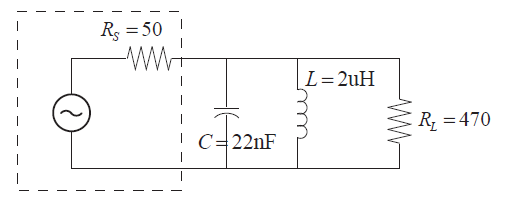
\includegraphics[scale=1]{04}
          
          \label{fig:04}
        \end{figure}
        
        

    \subsection{4.2 Atividade 2 – Filtros Passivos}
    
    \subsubsection{Filtro Passa-Baixas (FPB)}
        Esse experimento consistiu no projeto de um filtro passa-baixas RC com 
        as seguintes características: $f_c = 276 Hz$ e $C = 150 nF$. Foi então 
        plotada a resposta em frequência para esse circuito no intervalo de 15 
        Hz a 10 kHz. Plotou-se também o gráfico de fase do sinal onde é 
        possível observar a defasagem de fase e compará-la com a calculada 
        através do gráfico de Lissajous.

    \subsubsection{4.2.2 Filtro Passa-Altas (FPA)}
        O último experimento consistiu no projeto de um filtro passa-altas RC 
        com as seguintes características: $f_c = 5,2 kHz$ e $C = 150 nF$. O 
        sinal de saída foi analisado para uma faixa de frequência do sinal de 
        entrada entre 100 Hz e 100 kHz. Plotou-se então o gráfico de Lissajous 
        para analisar a defasagem do sinal.
        
        